
\documentclass[11pt]{exam} % https://www.ctan.org/pkg/exam?lang=en

\usepackage[lmargin=1.in,rmargin=1.in,tmargin=1.in,bmargin=1in]{geometry}
\usepackage{setspace}
\usepackage[pdftex]{graphicx}
\usepackage{titling}
\usepackage[
	pdfauthor={Brian Weinstein},
	pdftitle={Homework 2},
	bookmarks=true,
	colorlinks=true,
	linkcolor=blue,
	urlcolor=blue,
	citecolor=blue,
	pdftex,
	linktocpage=true
	]{hyperref}
\usepackage[textsize=tiny]{todonotes}
\usepackage{float}
\setlength\parindent{0pt}


\qformat{\textbf{Problem \thequestion: \thequestiontitle}\quad \hfill}


\pagestyle{headandfoot}
\runningheadrule
\firstpageheader{}{}{}
\runningheader{\thetitle}{\theauthor}{\thedate}
\firstpagefooter{}{\thepage}{}
\runningfooter{}{\thepage}{}





\usepackage{xcolor}
\usepackage{adjustbox}
\usepackage{verbatim}
\definecolor{shadecolor}{rgb}{.9, .9, .9}

\newenvironment{code}%
   {\par\noindent\adjustbox{margin=1ex,bgcolor=shadecolor,margin=0ex \medskipamount}\bgroup\minipage\linewidth\verbatim}%
   {\endverbatim\endminipage\egroup}

\newenvironment{codeSmall}%
   {\par\noindent\adjustbox{margin=1ex,bgcolor=shadecolor,margin=0ex \medskipamount}\bgroup\minipage\linewidth\verbatim\footnotesize}%
   {\endverbatim\endminipage\egroup}





\begin{document}


\title{STAT S4240 002, Homework 2}
\author{Brian Weinstein (bmw2148)}
\date{July 23, 2015}
\maketitle



\begin{questions}



\titledquestion{PCA}

\begin{parts}



\part Column means
\begin{code}
> apply(rawData, 2, mean)
       x1        x2        x3        x4        x5 
 6.049104 -8.277221  4.665532  7.914270 62.138753 
\end{code}
 
Row means
\begin{code}
> apply(rawData, 1, mean)
  [1]  -0.1277116  20.8162864  -8.8984358  25.5999204  -9.7472153
  [6]  64.0626702  22.0392371  23.3914888  31.7598224 -13.8680290
...
 [91]   1.2105932  21.2145724  -8.4896595  19.0639963  20.9767512
 [96]   3.5962333  22.3461063   0.7145014   6.3080005  64.8829556
\end{code}

The nonzero column means indicate that each variable isn't centered. In this context the row means are just the average of the coordinates for each observation. 
 
 
\part Empirical covariance matrix
\begin{code}
          x1         x2        x3        x4        x5
x1  72.96417  -83.90858  53.23708  120.1162  568.4105
x2 -83.90858  110.89101 -63.89570 -115.9430 -817.3388
x3  53.23708  -63.89570  39.60282   83.7386  445.2511
x4 120.11620 -115.94304  83.73860  232.1333  683.5587
x5 568.41046 -817.33884 445.25112  683.5587 6288.8569
\end{code}

The diagonal values tell us the variance of the variable indicated in the column (or equivalently, the row). The off-diagonal elements indicate the covariance between the two variables that intersect at that element.

\part The eigenvalues and eigenvectors of the empirical covariance matrix \texttt{sig}:
\begin{code}
> eigen(sig)
$values
[1] 6.557348e+03 1.868951e+02 2.038354e-01 9.775594e-04 9.373658e-05

$vectors
            [,1]       [,2]         [,3]        [,4]        [,5]
[1,]  0.09009603 -0.3247102 -0.383470773  0.82286709  0.24957150
[2,] -0.12797842  0.1364755  0.227047683 -0.11412319  0.94890526
[3,]  0.07028767 -0.1941349  0.894987159  0.37278501 -0.13191135
[4,]  0.11077853 -0.9008231 -0.019718518 -0.40719485  0.10024632
[5,]  0.97892389  0.1636064  0.002946326 -0.07133967  0.09921159
\end{code}

where the eigenvectors are represented as columns in the \texttt{\$vectors} component.

Since it's a symmetric matrix, \texttt{sig} has the same left eigenvectors as right eigenvectors.

\part The loadings are the eigenvectors (see part c). The scores are:
\begin{code}
> data%*%t(evecs)
               [,1]          [,2]         [,3]         [,4]        [,5]
  [1,]  -25.9233299  -50.96254603  -4.06557021  -8.91350845 -10.7755359
  [2,]   13.3064897   13.56908728   6.16049505   0.82185440   4.8621981
  [3,]  -37.6872799  -93.30323983  -1.02562352 -18.15040050 -16.3848300
...
 [98,]  -27.0931525  -38.88284377  -8.26671502  -5.26069573 -10.6527232
 [99,]  -13.1627026  -31.46409161  -1.20277265  -5.83681744  -5.6197025
[100,]   85.7232563  184.73133084  10.16179165  33.54024954  36.1560703
\end{code}

\part Proportion of variance explained

\begin{figure}[H]
	\centering
	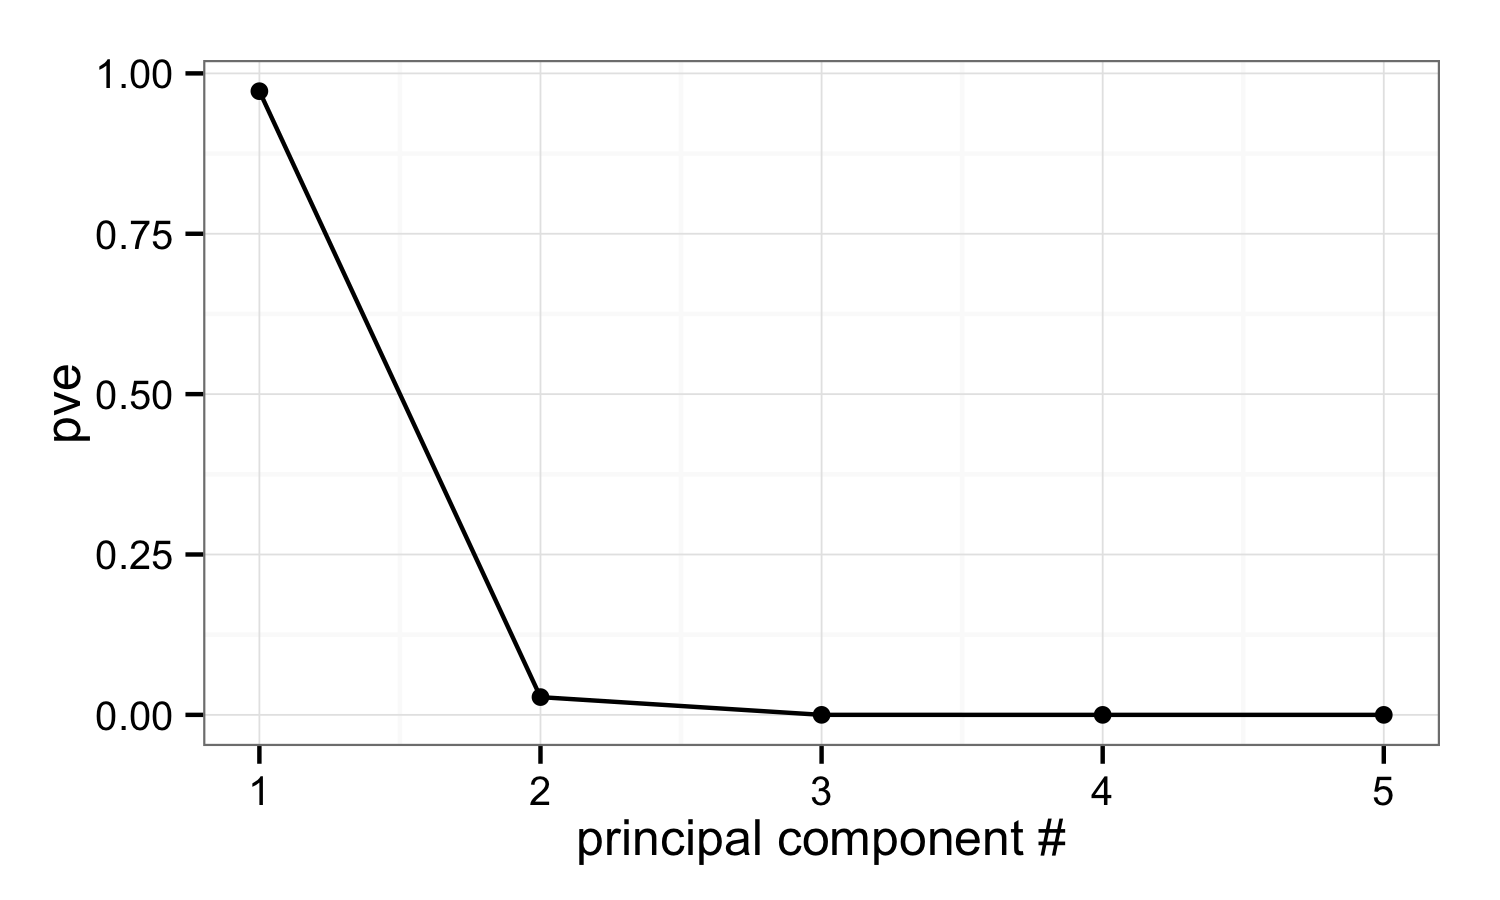
\includegraphics[width=5in]{1e.png}
	%\caption{}
	%\label{fig:figName}
\end{figure}

We only need one principal component. PC \#1 accounts for 97\% of the variance on its own, and including any additional PCs introduces more complexity than it's worth.

\part The scores for the new observations:

\begin{code}
           [,1]       [,2]      [,3]        [,4]        [,5]
[1,] -16.855658 -66.790142  6.776900 -15.3066224  -8.5649268
[2,]   4.861635  26.789815 -3.710359   6.3835809   2.7072847
[3,]   2.536648   1.355434  1.590414  -0.2530266   0.8012362
[4,] -30.863147 -57.879087 -5.570018  -9.7920953 -12.6610309
[5,] -11.787862 -14.507653 -3.653059  -1.8812777  -4.6755677
\end{code}


\part Coordinates of the projections in the original space:

\begin{code}
           [,1]       [,2]     [,3]    [,4]     [,5]
[1,] -10.871807 -38.241645 4.665532 7.91427 62.13875
[2,]  37.567018  66.568511 4.665532 7.91427 62.13875
[3,]  16.460691  25.729053 4.665532 7.91427 62.13875
[4,]   5.978194 -41.185647 4.665532 7.91427 62.13875
[5,]   1.857621  -6.945432 4.665532 7.91427 62.13875
\end{code}

Euclidean distance from the original data points.
\begin{code}
[1] 81.49181
[1] 88.13304
[1] 36.01572
[1] 79.53924
[1] 19.04255
\end{code}


\part The error vectors are more or less orthogonal to the direction of the first principal component. This is because the error vectors are defined as the direction from the original points to their \textit{orthogonal projections} onto the reduced-dimension space, which is primarily captured by the first PC.


\end{parts}




\titledquestion{PCA with Yale Faces B}


\begin{parts}

\part The matrix is 152 rows by 32,256 columns. Each row of the matrix is one photograph (38 subjects with 4 views each), and each column is a pixel in each image (originally 192 x 168).

\part Mean face:

\begin{figure}[H]
	\centering
	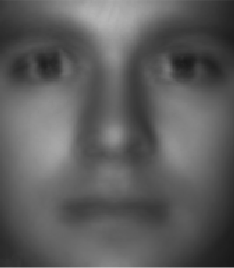
\includegraphics[width=168px]{2b_mean_face_fixed.png}
	%\caption{}
	%\label{fig:figName}
\end{figure}

\part Proportion of variance explained

\begin{figure}[H]
	\centering
	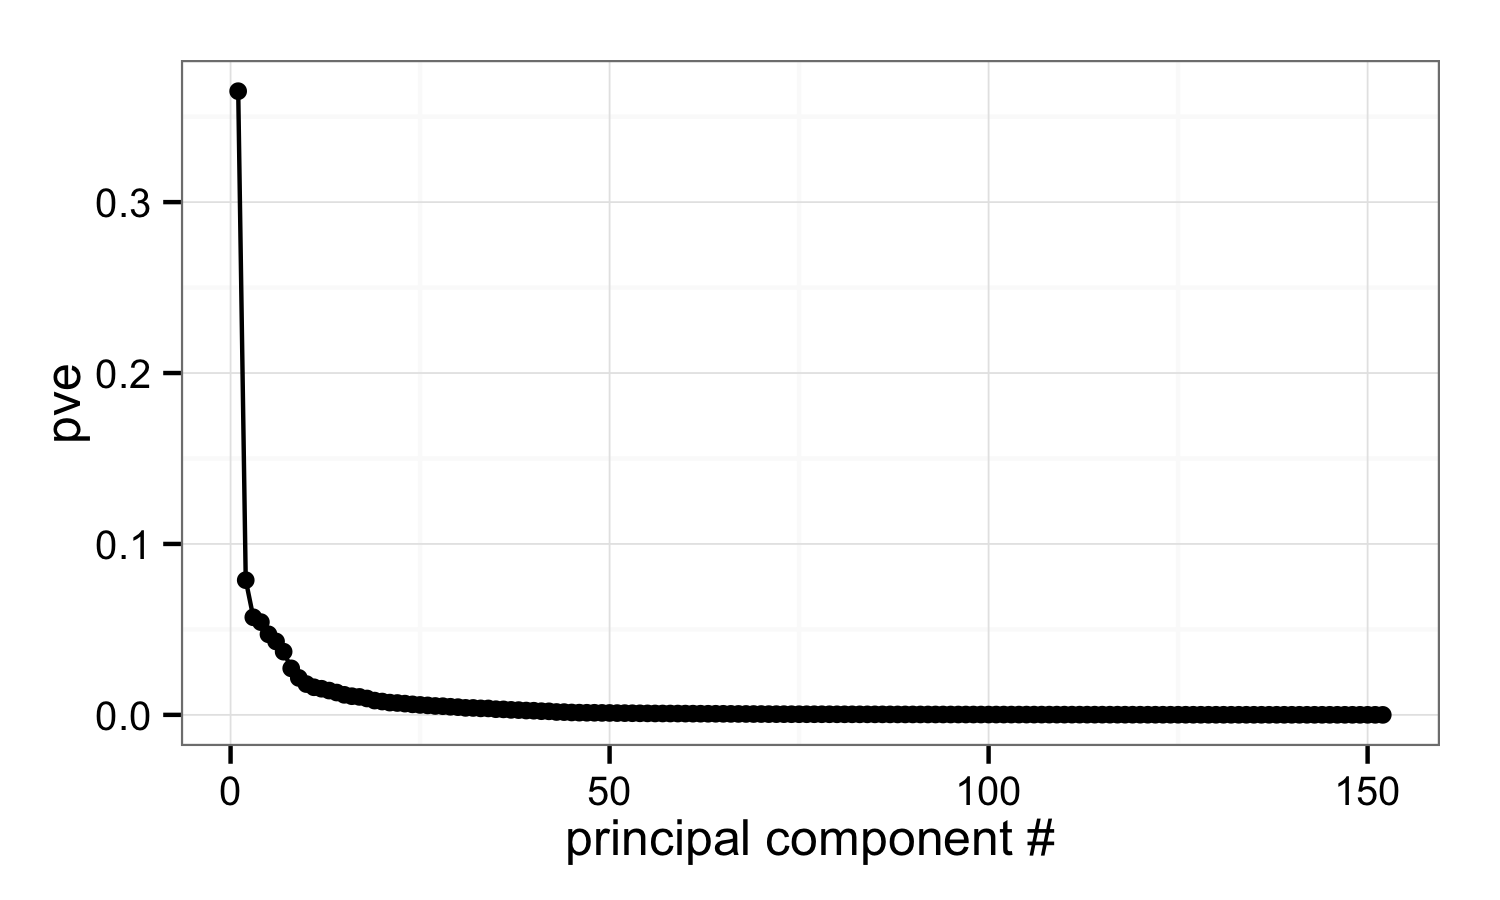
\includegraphics[width=5in]{2c.png}
	%\caption{}
	%\label{fig:figName}
\end{figure}


\part The first 9 eigenfaces are the (constructed) images that capture the most variable aspects of the faces in the dataset. The first image amplifies the most variable pixels in the original images, the second image amplifies the most variable pixels in a direction orthogonal to the first principal component, the third the most variable pixels in a direction orthogonal to the first two principal components, etc.

\begin{figure}[H]
	\centering
	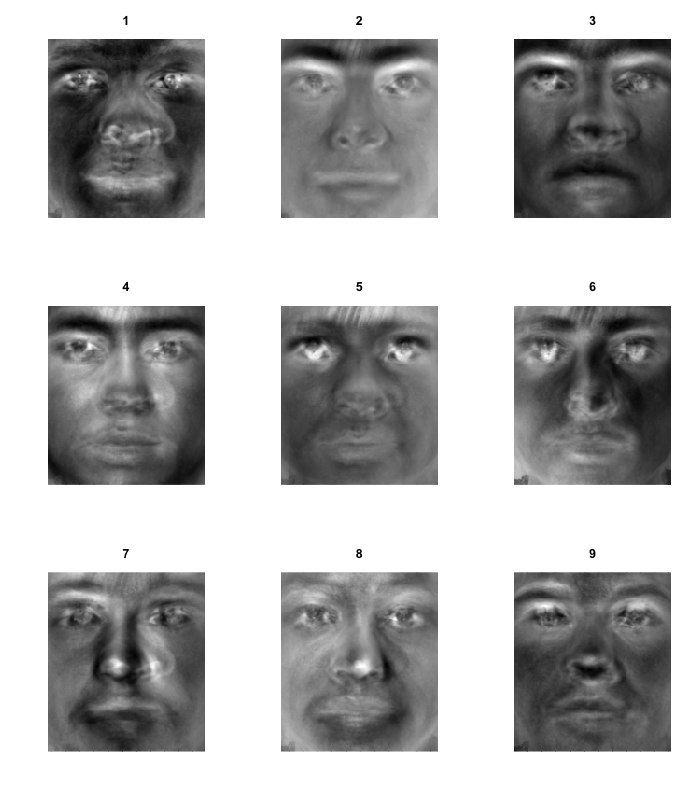
\includegraphics[width=5in]{2d_pca_faces.png}
	%\caption{}
	%\label{fig:figName}
\end{figure}




\part Reconstructing \texttt{yaleB05\_P00A+010E+00.pgm} using 24 eigenfaces:

\begin{figure}[H]
	\centering
	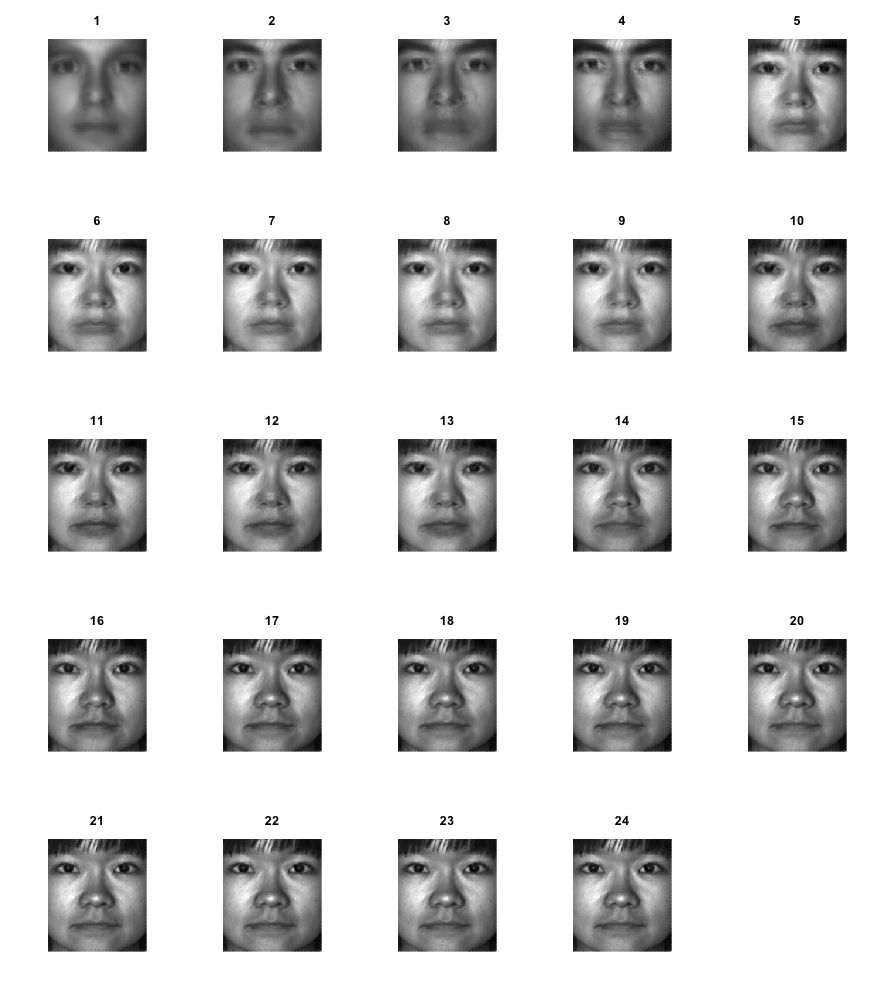
\includegraphics[width=6in]{2e_faces24.png}
	%\caption{}
	%\label{fig:figName}
\end{figure}

Reconstructing \texttt{yaleB05\_P00A+010E+00.pgm} using 120 eigenfaces, in steps of 5:

\begin{figure}[H]
	\centering
	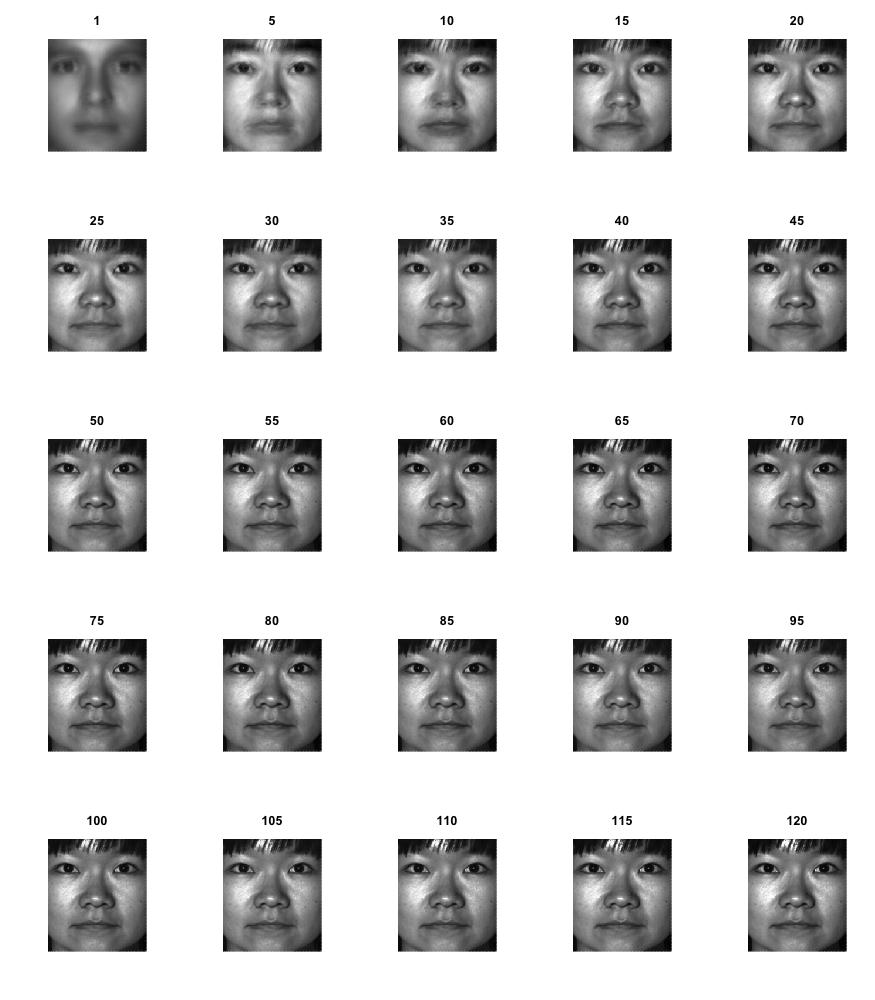
\includegraphics[width=6in]{2e_faces120.png}
	%\caption{}
	%\label{fig:figName}
\end{figure}

After incorporating 14 or 15 eigenfaces, the person is relatively recognizable




\part After removing the images of Subject 1, re-running PCA on the reduced dataset, and then reconstructing a photo of Subject 1 using the principal components; the reconstructed photo (right) has similar features to the original (left), but it's definitely not a recognizable image.

It doesn't look much like the original image because we excluded all photos of Subject 1 before computing the principal components. As such, the features present in the subject's original photos weren't incorporated into either the ``mean face'' or into the principal components.

\begin{figure}[H]
	\centering
	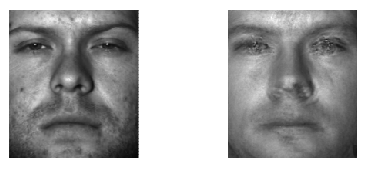
\includegraphics[width=5in]{2f_cropped.png}
	%\caption{}
	%\label{fig:figName}
\end{figure}


\end{parts}


\titledquestion{\href{http://www-bcf.usc.edu/~gareth/ISL/}{James} 3.7.3}

\begin{parts}

\part iii. For a fixed value of IQ and GPA, males earn more on average than females provided that the GPA is high enough.
$$Salary=50+(20*GPA)+(0.07*IQ)+(35*I_{female})+(0.01*GPA*IQ)+(-10*GPA*I_{female})$$
Thus, once GPA is high enough, the $(-10*GPA*I_{female})$ term dominates and reduces female salary.

\part For a female ($I_{female}=1$) with $IQ=110$ and $GPA=4.0$, the salary (in thousands of dollars) is predicted to be:
$$Salary=50+(20*4.0)+(0.07*110)+(35*1)+(0.01*4.0*110)+(-10*4.0*1)=137.1$$

\part False. A small coefficient for the GPA/IQ interaction term does not mean there's little \textit{evidence} of an interaction effect. To determine how strong the evidence of interaction is, we should look at the p-value of the term's coefficient $\beta_4$. If the term is significant, the small coefficient indicates that the interaction between GPA and IQ has little effect on Salary.

\end{parts}


\titledquestion{\href{http://www-bcf.usc.edu/~gareth/ISL/}{James} 3.7.4}

\begin{parts}

\part If the true relationship is linear (with a random error term), the training RSS for the cubic regression will be lower than the training RSS for the linear regression. This is because, while using training data, a more flexible model (e.g., cubic vs linear) will always fit better than a less flexible one.

\part The testing RSS, on the other hand, will be lower for the linear regression than the testing RSS for the cubic regression. By using the cubic regression on a truly linear relationship, the RSS will indicate that we overfit the data.

\part If we know that the relationship isn't linear, but we don't know how far it is from linear, we'll still have a lower RSS for the cubic regression than for the linear regression. As noted in part (a), this is because a more flexible model will always reduce the training RSS more than a less flexible one.

\part If we again know that the relationship isn't linear, but we don't know how far it is from linear, it's not clear which model will have a lower test RSS. We need to know if the model is closer to linear or closer to cubic to determine which model would have a lower test RSS.

\end{parts}




\titledquestion{$k$NN: Leave One Out Cross Validation}

\begin{parts}

\part Distances among all pairs of points (cleaned up the output in the interest of space)

\begin{codeSmall}
            1          2          3          4          5          6          7
2  0.42225823                                                                  
3  4.89266476 4.48324140                                                       
4  3.52558292 3.28052936 3.03849890                                            
5  1.61575766 1.20175523 3.28214677 2.56169484                                 
6  4.01731301 3.75476341 2.84914128 0.51893201 2.95233169                      
7  4.99313534 4.60912059 0.86746538 2.51269749 3.44543841 2.21211835           
8  4.73564051 4.37259481 1.33525544 1.99045562 3.25906027 1.66138958 0.55781634
9  4.82178404 4.41884121 0.27098224 2.80100836 3.22339706 2.59295742 0.61614524
10 4.90836910 4.56390437 1.73066927 1.88888700 3.49657042 1.47861570 0.89619151
11 3.24398876 3.23168183 4.91467055 1.93685219 3.22349344 2.32967788 4.44684306
12 6.77417716 6.39323343 2.19303519 3.96528020 5.23030556 3.52898864 1.78541086
13 4.28583792 3.87263766 0.63295157 2.78924724 2.67100051 2.70576828 1.21457856
14 0.37376933 0.20171780 4.62203155 3.48158451 1.34256539 3.95451105 4.77254054
15 5.92113938 5.59929777 2.58515802 2.59937089 4.57968745 2.09038441 1.73190885
16 1.27492496 0.86782992 3.61795545 2.65949840 0.34834264 3.08734143 3.74901047
17 2.83507180 2.63923900 3.51427136 0.78677953 2.14660056 1.30428651 3.12564303
18 5.04607936 4.64334911 0.31803000 2.95278924 3.44794848 2.71458849 0.59668630
19 4.36372255 4.03808157 2.00769642 1.26832777 3.03296584 0.90197629 1.31400902
20 4.98088347 4.59654436 0.85615905 2.50955789 3.43224904 2.21170478 0.01525788

            8          9         10         11         12         13         14                                                                        
9  1.06450035                                                                  
10 0.41661801 1.46210862                                                       
11 3.92716052 4.69433257 3.80132633                                            
12 2.08868023 2.11442621 2.07847065 5.85822435                                 
13 1.48588658 0.68297525 1.90162337 4.57198474 2.79142747                      
14 4.54812111 4.56594343 4.74688312 3.40818552 6.55769923 4.00594363           
15 1.48137311 2.34648069 1.12127822 4.32465226 1.78541534 2.91451535 5.78862417
16 3.53387540 3.55106146 3.74868164 3.09628992 5.53424388 3.01141347 1.02358784
17 2.64776724 3.30661926 2.61367917 1.42821021 4.68905906 3.14684750 2.84047751
18 1.11856965 0.22456208 1.48857091 4.86177365 1.91170442 0.88008662 4.79049829
19 0.76003405 1.74177978 0.62733983 3.19454523 2.70506597 1.98005600 4.22719726
20 0.55965989 0.60354012 0.90297392 4.44322841 1.79838792 1.19965611 4.75974994

           15         16         17         18         19                                                    
16 4.81222179                                            
17 3.38421301 2.15185288                                 
18 2.28313471 3.77555821 3.48682301                      
19 1.56143054 3.25446038 1.98646549 1.84007232           
20 1.74525321 3.73620047 3.11992410 0.58810214 1.31437805
\end{codeSmall}


\part Using data point 1 as the testing set and the remaining points as a training set, $k$NN for $k \in \{1, 2, \ldots, 10\}$ yields the following testing MSE ($MSE^{k,1}_{test}$), and training MSE ($MSE^{k,1}_{train}$):

\begin{code}
   kValue      testMSE   trainMSE
1       1 0.0196656396 0.00000000
2       2 0.0268217849 0.02985241
3       3 0.0152777998 0.04586316
4       4 0.0014688370 0.06450685
5       5 0.0032978182 0.06215975
6       6 0.0008362937 0.07557705
7       7 0.0192632625 0.08332753
8       8 0.0656325812 0.10100542
9       9 0.0964741491 0.10691977
10     10 0.1647239008 0.13030996
\end{code}


\part Now performing leave one out cross validation, the testing and training MSEs are determined as
$$MSE^{k}_{test}=\frac{1}{n}\sum_{i=1}^{n}MSE^{k,i}_{test}\quad\quad\quad
MSE^{k}_{train}=\frac{1}{n}\sum_{i=1}^{n}MSE^{k,i}_{train}$$

where $i$ is the index of the data point left out and $n=20$, the size of our dataset.


\begin{code}
   kValue    testMSE   trainMSE
1       1 0.11442243 0.00000000
2       2 0.09968107 0.02880520
3       3 0.10780903 0.04563393
4       4 0.08949504 0.05918676
5       5 0.10361356 0.06048102
6       6 0.09665278 0.07129727
7       7 0.10652029 0.07454968
8       8 0.12116962 0.08717699
9       9 0.12600534 0.09846322
10     10 0.14395572 0.11061502
\end{code}


\part We should use the $k$ value that minimizes the test MSE, which here is $k=4$.

\begin{figure}[H]
	\centering
	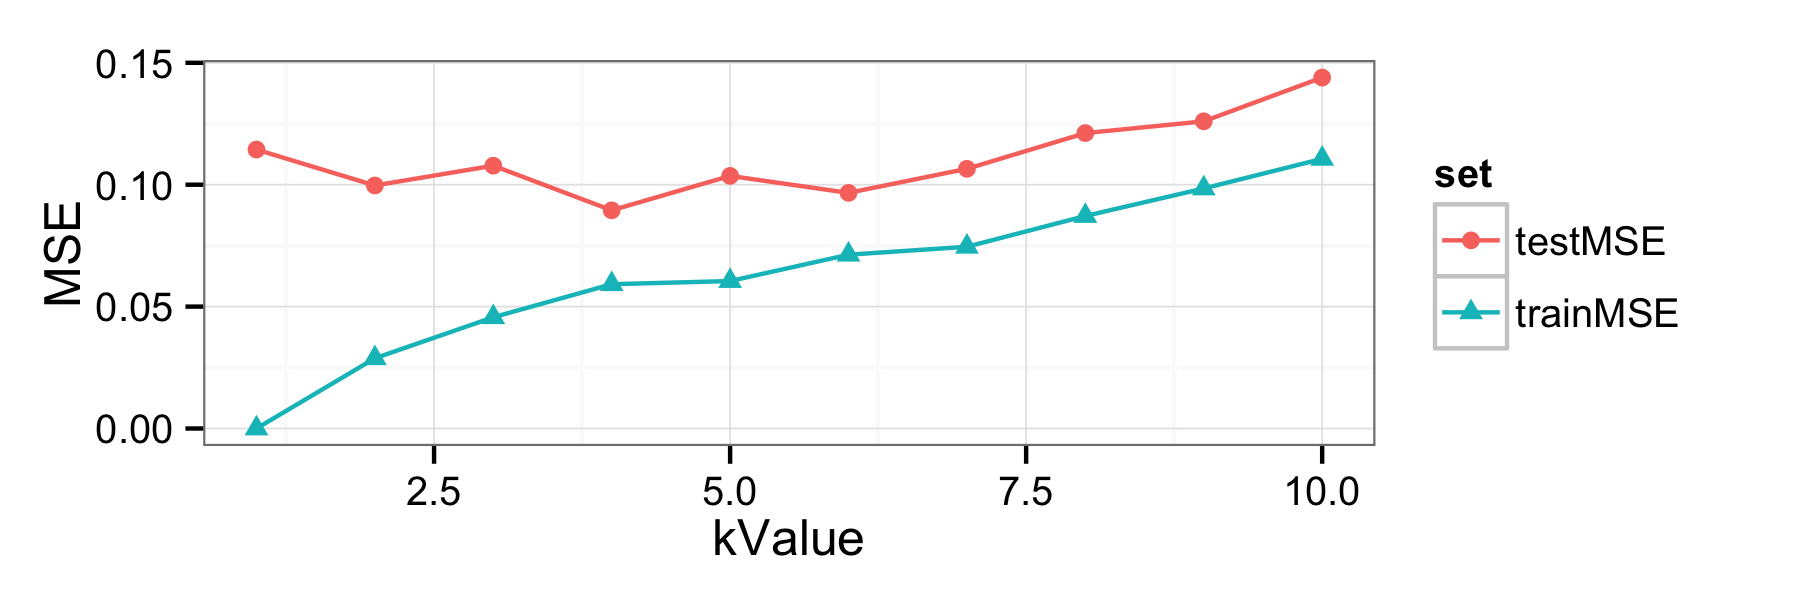
\includegraphics[width=6in]{5d.png}
	%\caption{}
	%\label{fig:figName}
\end{figure}

In choosing a value of $k$ that generates the best model, we should always use the one that minimizes the testing error, and never the training error. We can't assess model accuracy using the training error since, by construction, the training error will decrease as model flexibility increases (i.e., as $k$ decreases). We need to assess the model using \textit{previously unseen data}, which, in this case, means minimizing the testing error.

\end{parts}


\titledquestion{Facial Recognition with $1$NN and PCA}

\begin{parts}

\part First five files in the training set:
\begin{code}
> head(subjectViewLabels[sort(ind_train_6a), ], 5)
  subject         view                  key
1 yaleB01 P00A+000E+00 yaleB01/P00A+000E+00
2 yaleB01 P00A+005E+10 yaleB01/P00A+005E+10
3 yaleB01 P00A+005E-10 yaleB01/P00A+005E-10
4 yaleB01 P00A+010E+00 yaleB01/P00A+010E+00
6 yaleB02 P00A+005E+10 yaleB02/P00A+005E+10
\end{code}

First five files in the testing set:
\begin{code}
> head(subjectViewLabels[sort(ind_test_6a), ], 5)
   subject         view                  key
5  yaleB02 P00A+000E+00 yaleB02/P00A+000E+00
12 yaleB03 P00A+010E+00 yaleB03/P00A+010E+00
18 yaleB05 P00A+005E+10 yaleB05/P00A+005E+10
20 yaleB05 P00A+010E+00 yaleB05/P00A+010E+00
21 yaleB06 P00A+000E+00 yaleB06/P00A+000E+00
\end{code}

\part In my model, it looks like I correctly classified all 31 test photos. This isn't entirely surprising, though, since each test subject had at least one photo of them present in the training group.


%\part
%
%\part
%
%\part


\end{parts}



\end{questions}

%\listoftodos

\end{document}